\documentclass[12pt]{report}

\usepackage{geometry}
\usepackage[T1]{fontenc}
\usepackage[utf8]{inputenc}
\usepackage[francais]{babel}

\usepackage{graphicx}
\usepackage{lmodern}

\geometry{margin=2cm}


\begin{document}

\thispagestyle{empty}
\noindent
\includegraphics[width=0.25\textwidth]{enseirb-matmeca}

\vspace{\stretch{1}}

\begin{center}
	\Huge{\textbf{Rapport de projet SGBD :}}
	
	\Huge{\textbf{Bandes dessinées}}
\end{center}

\vspace{\stretch{2}}

\begin{tabular}{r@{:~}l}
	\textbf{Auteurs} & \textit{David Bitonneau, Ludovic Hofer, Benoît Ruelle}\\
	\textbf{Encadrants} & \textit{Mme. Allyx Fontaine, M. Sylvain Lombardy,
M. Mohamed Mosbah}\\
\end{tabular}

\vspace{\stretch{1}}

\begin{center}Deuxième année, filière informatique

Date : \today\end{center}

\newpage

\section{Introduction}

\emph{re-decrire le sujet en detaillant}

L'objectif du projet est de mettre en œuvre, sur un cas pratique, les notions
et les méthodes vues dans le module de SGBD. L'application effectuée ici est
liée à la gestion de bandes dessinées.

Dans ce rapport, la base de données est décrite de sa conception à son
utilisation, en passant par son implémentation. Les choix effectués par le
groupe de projet sont détaillés et justifiés lorsque cela est nécessaire.

\section{Modélisation des données}

\emph{Justifier vos choix/hypotheses avec du texte}

\subsection{Description du contexte de l'application (entités, associations, règles de gestion)}

\paragraph{}
L'application doit permettre la gestion de bandes dessinées à partir des
informations suivantes :

\begin{itemize}
	\item Chaque volume de bande dessinée est soit un album, soit une revue.
	\item Tout volume a un éditeur, et une année d’édition.
	\item Un album peut éventuellement appartenir à une collection, et dans ce cas, il
		peut avoir un numéro dans cette collection. Deux albums de la même collection
		ont forcément le même éditeur.
	\item Un volume a un titre, qui est soit le titre de l'album, soit celui de la
		revue ; dans le cas de la revue, elle a aussi un numéro.
	\item Un volume peut contenir plusieurs histoires.
	\item Chaque histoire a un titre et une année de (première) parution ; elle a un
		ou plusieurs auteurs, chacun de ces auteurs s’occupant du dessin ou du
		scénario (ou des deux).
	\item Une même histoire peut apparaître dans différents volumes ; on veut pouvoir
		annoter la présence d’une histoire dans un volume ("Première publication",
		"Pages 15 à 22", "Version longue", etc.).
	\item Une histoire peut appartenir à une série et dans ce cas elle peut avoir un
		numéro de série.
\end{itemize}

On considère qu'une revue est un ensemble de numéros de la revue et que
l'éditeur d'une revue peut varier dans le temps.

\paragraph{}
La lecture de ces informations fait ressortir les entités suivantes :
\begin{itemize}
	\item volume ;
	\item album ;
	\item revue ;
	\item éditeur ;
	\item collection ;
	\item histoire ;
	\item série ;
	\item auteur.
\end{itemize}

\paragraph{}
Le schéma entité-association suivant montre les relations entre ces
différentes entités :

\noindent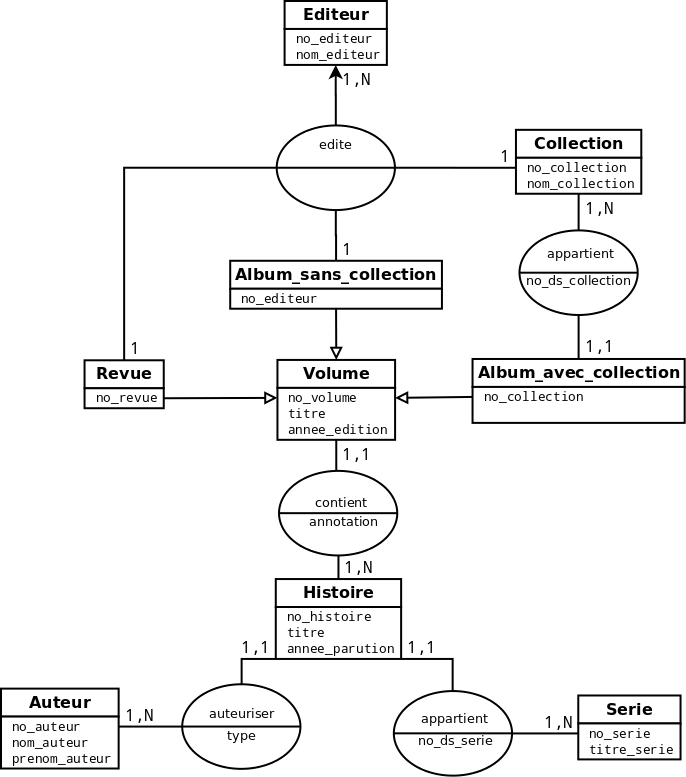
\includegraphics[width=\textwidth]{schema-entite-association}

\subsection{Liste des opérations prévues sur la base (consultation, mise à
jour, etc.}

\section{Schéma relationnel :}

\subsection{Passage au relationnel}

\subsection{Contraintes d'intégrité, dépendances fonctionnelles}

\subsection{Schéma relationnel en 3e forme normale}

\noindent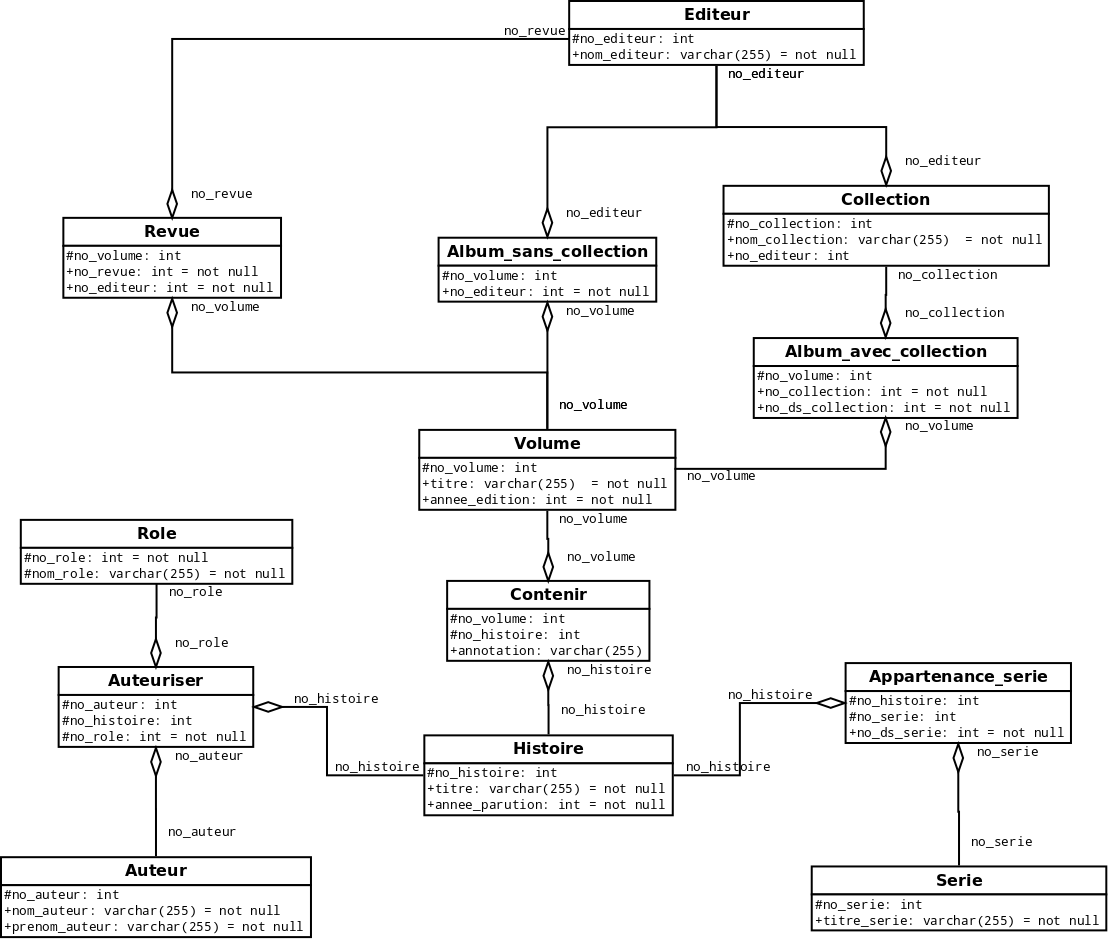
\includegraphics[width=\textwidth]{schema-relation}

\section{Implémentation }
-> choix de MySQL

\subsection{Création de la base de données, en prenant en compte les contraintes d'intégrité (scripts de création, suppression, insertion)}

\subsection{Implémentation des commandes SQL réalisant les opérations retenues}

\emph{Lister les requetes importantes}

\section{Utilisation :}

\subsection{Description de l'environnement d'exécution}

\emph{Decrire l'environnement et l'installation}

\subsection{Notice d'utilisation}

\subsection{Description des interfaces éventuelles (Shell, JDBC, PHP, etc.)}

\end{document}
